% What a Consensus result must pass before the assistant may cite it.
% ---------------------------------------------------------------------------
% style.tex --- shared preamble for every figure in book/figures/tikz/
%
% One style for all figures: Latin Modern, thin black lines, a light grey
% fill, and one accent colour used only to mark what is untrusted or wrong.
% Build with scripts/build_figures.sh; see book/figures/README.md.
% ---------------------------------------------------------------------------
\documentclass[tikz,border=6pt]{standalone}
\usepackage[T1]{fontenc}
\usepackage{lmodern}
\usetikzlibrary{arrows.meta,positioning,shapes.geometric,calc,fit,backgrounds}

\hyphenpenalty=10000   % short lines in boxes: ragged, never hyphenated

\definecolor{lightgrey}{gray}{0.92}
\definecolor{accent}{HTML}{9B2D20}

\tikzset{
  every picture/.style={
    line width=0.6pt,
    font=\small,
    >={Stealth[length=5pt,width=4pt]},
    node distance=14pt and 24pt,
  },
  % shapes
  box/.style={draw, rectangle, inner xsep=8pt, inner ysep=5pt,
              minimum height=22pt, align=center},
  grey/.style={box, fill=lightgrey},
  rounded/.style={box, rounded corners=9pt},
  decision/.style={draw, diamond, aspect=2.4, inner sep=1.5pt, align=center},
  group/.style={draw, dashed, rounded corners=5pt, inner sep=7pt},
  % text
  tag/.style={font=\footnotesize, align=center, inner sep=2pt},
  note/.style={font=\footnotesize\itshape, align=center, inner sep=2pt},
  code/.style={font=\small\ttfamily},
  codetag/.style={font=\footnotesize\ttfamily, align=center, inner sep=2pt},
  title/.style={font=\small\scshape, align=center, inner sep=2pt},
  % lines
  arrow/.style={->},
  back/.style={->, dashed},
  thin/.style={line width=0.4pt, gray},
  % the one accent, for what is untrusted, wrong or missing
  bad/.style={accent},
  badbox/.style={box, draw=accent, text=accent},
}

\begin{document}
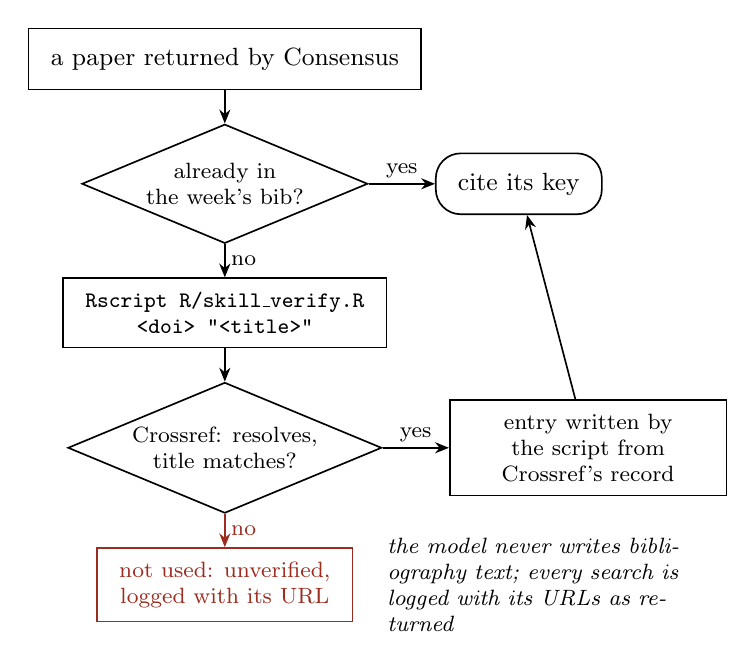
\begin{tikzpicture}[node distance=12pt and 24pt]
  \node[box] (res) {a paper returned by Consensus};
  \node[decision, below=of res, font=\footnotesize] (inbib) {already in\\the week's bib?};
  \node[rounded, right=of inbib] (cite) {cite its key};
  \node[box, below=of inbib, font=\footnotesize\ttfamily, align=center] (ver) {Rscript R/skill\_verify.R\\<doi> "<title>"};
  \node[decision, below=of ver, font=\footnotesize] (ok) {Crossref: resolves,\\title matches?};
  \node[box, right=of ok, text width=84pt, align=center, font=\footnotesize] (entry) {entry written by the script from Crossref's record};
  \node[badbox, below=of ok, font=\footnotesize, align=center] (no) {not used: unverified,\\logged with its URL};
  \draw[->] (res) -- (inbib);
  \draw[->] (inbib) -- node[tag, above] {yes} (cite);
  \draw[->] (inbib) -- node[tag, right] {no} (ver);
  \draw[->] (ver) -- (ok);
  \draw[->] (ok) -- node[tag, above] {yes} (entry);
  \draw[->, bad] (ok) -- node[tag, right, text=accent] {no} (no);
  \draw[->] (entry) -- (cite);
  \node[note, right=10pt of no.east, anchor=west, text width=120pt, align=left]
    {the model never writes bibliography text; every search is logged with its URLs as returned};
\end{tikzpicture}
\end{document}
